\documentclass[a4paper,11pt]{article}
\usepackage{fullpage}
\usepackage[latin1]{inputenc}
\usepackage[T1]{fontenc}
\usepackage[normalem]{ulem}
\usepackage[english]{babel}
\usepackage{listings,babel}
\lstset{breaklines=true,basicstyle=\ttfamily}
\usepackage{graphicx}
\usepackage{moreverb}
\usepackage{float}
\usepackage{url}
\usepackage{tabularx}

\title{Milkymist system reference manual}
\author{S\'ebastien Bourdeauducq}
\date{\today}
\begin{document}
\maketitle{}
\section{What is Milkymist}
The goal of the project is to develop a small stand-alone board that is capable of rendering MilkDrop presets in real time from an audio input (analog or digital), and displaying them on a VGA screen.

Open source components have been used as much as possible, and therefore a system-on-chip implemented in a FPGA has been chosen for meeting this goal as well as simplifying the PCB. Only a few components need to be added for a minimal video synthesis board:
\begin{itemize}
\item Off-chip memory
\item VGA DAC
\item Microphone and audio ADC
\item Debug console
\end{itemize}

\section{Supported boards}
\subsection{Xilinx ML401 development board}
This board is equipped with a Virtex-4 FPGA (XC4VLX25). Milkymist can use the on-board peripherals of the ML401:
\begin{itemize}
\item VGA output (Analog Devices ADV7125KST50 3x8-bit D/A converter)
\item AC'97 audio codec (National Semiconductor LM4550)
\item CF card slot (through Xilinx SystemACE)
\item RS232 port
\item LCD screen (Lumex LCM-S01602DTR/M, HD44780-compatible)
\item LEDs
\item Buttons
\item Parallel flash
\item DDRAM (two Infineon HYB25D256160BT-7 chips)
\end{itemize}

\subsection{Avnet Spartan-3A evaluation kit}
This board is equipped with a Spartan-3A XC3S400A chip. Because of the limited FPGA capacity and the small number of on-board peripherals, support for this board is only for educational and evaluation purposes.

The following peripherals are supported:
\begin{itemize}
\item RS232 port
\item LEDs
\item Buttons
\item Parallel flash
\end{itemize}

\section{Components and bus architecture}

\begin{figure}[H]
\centering
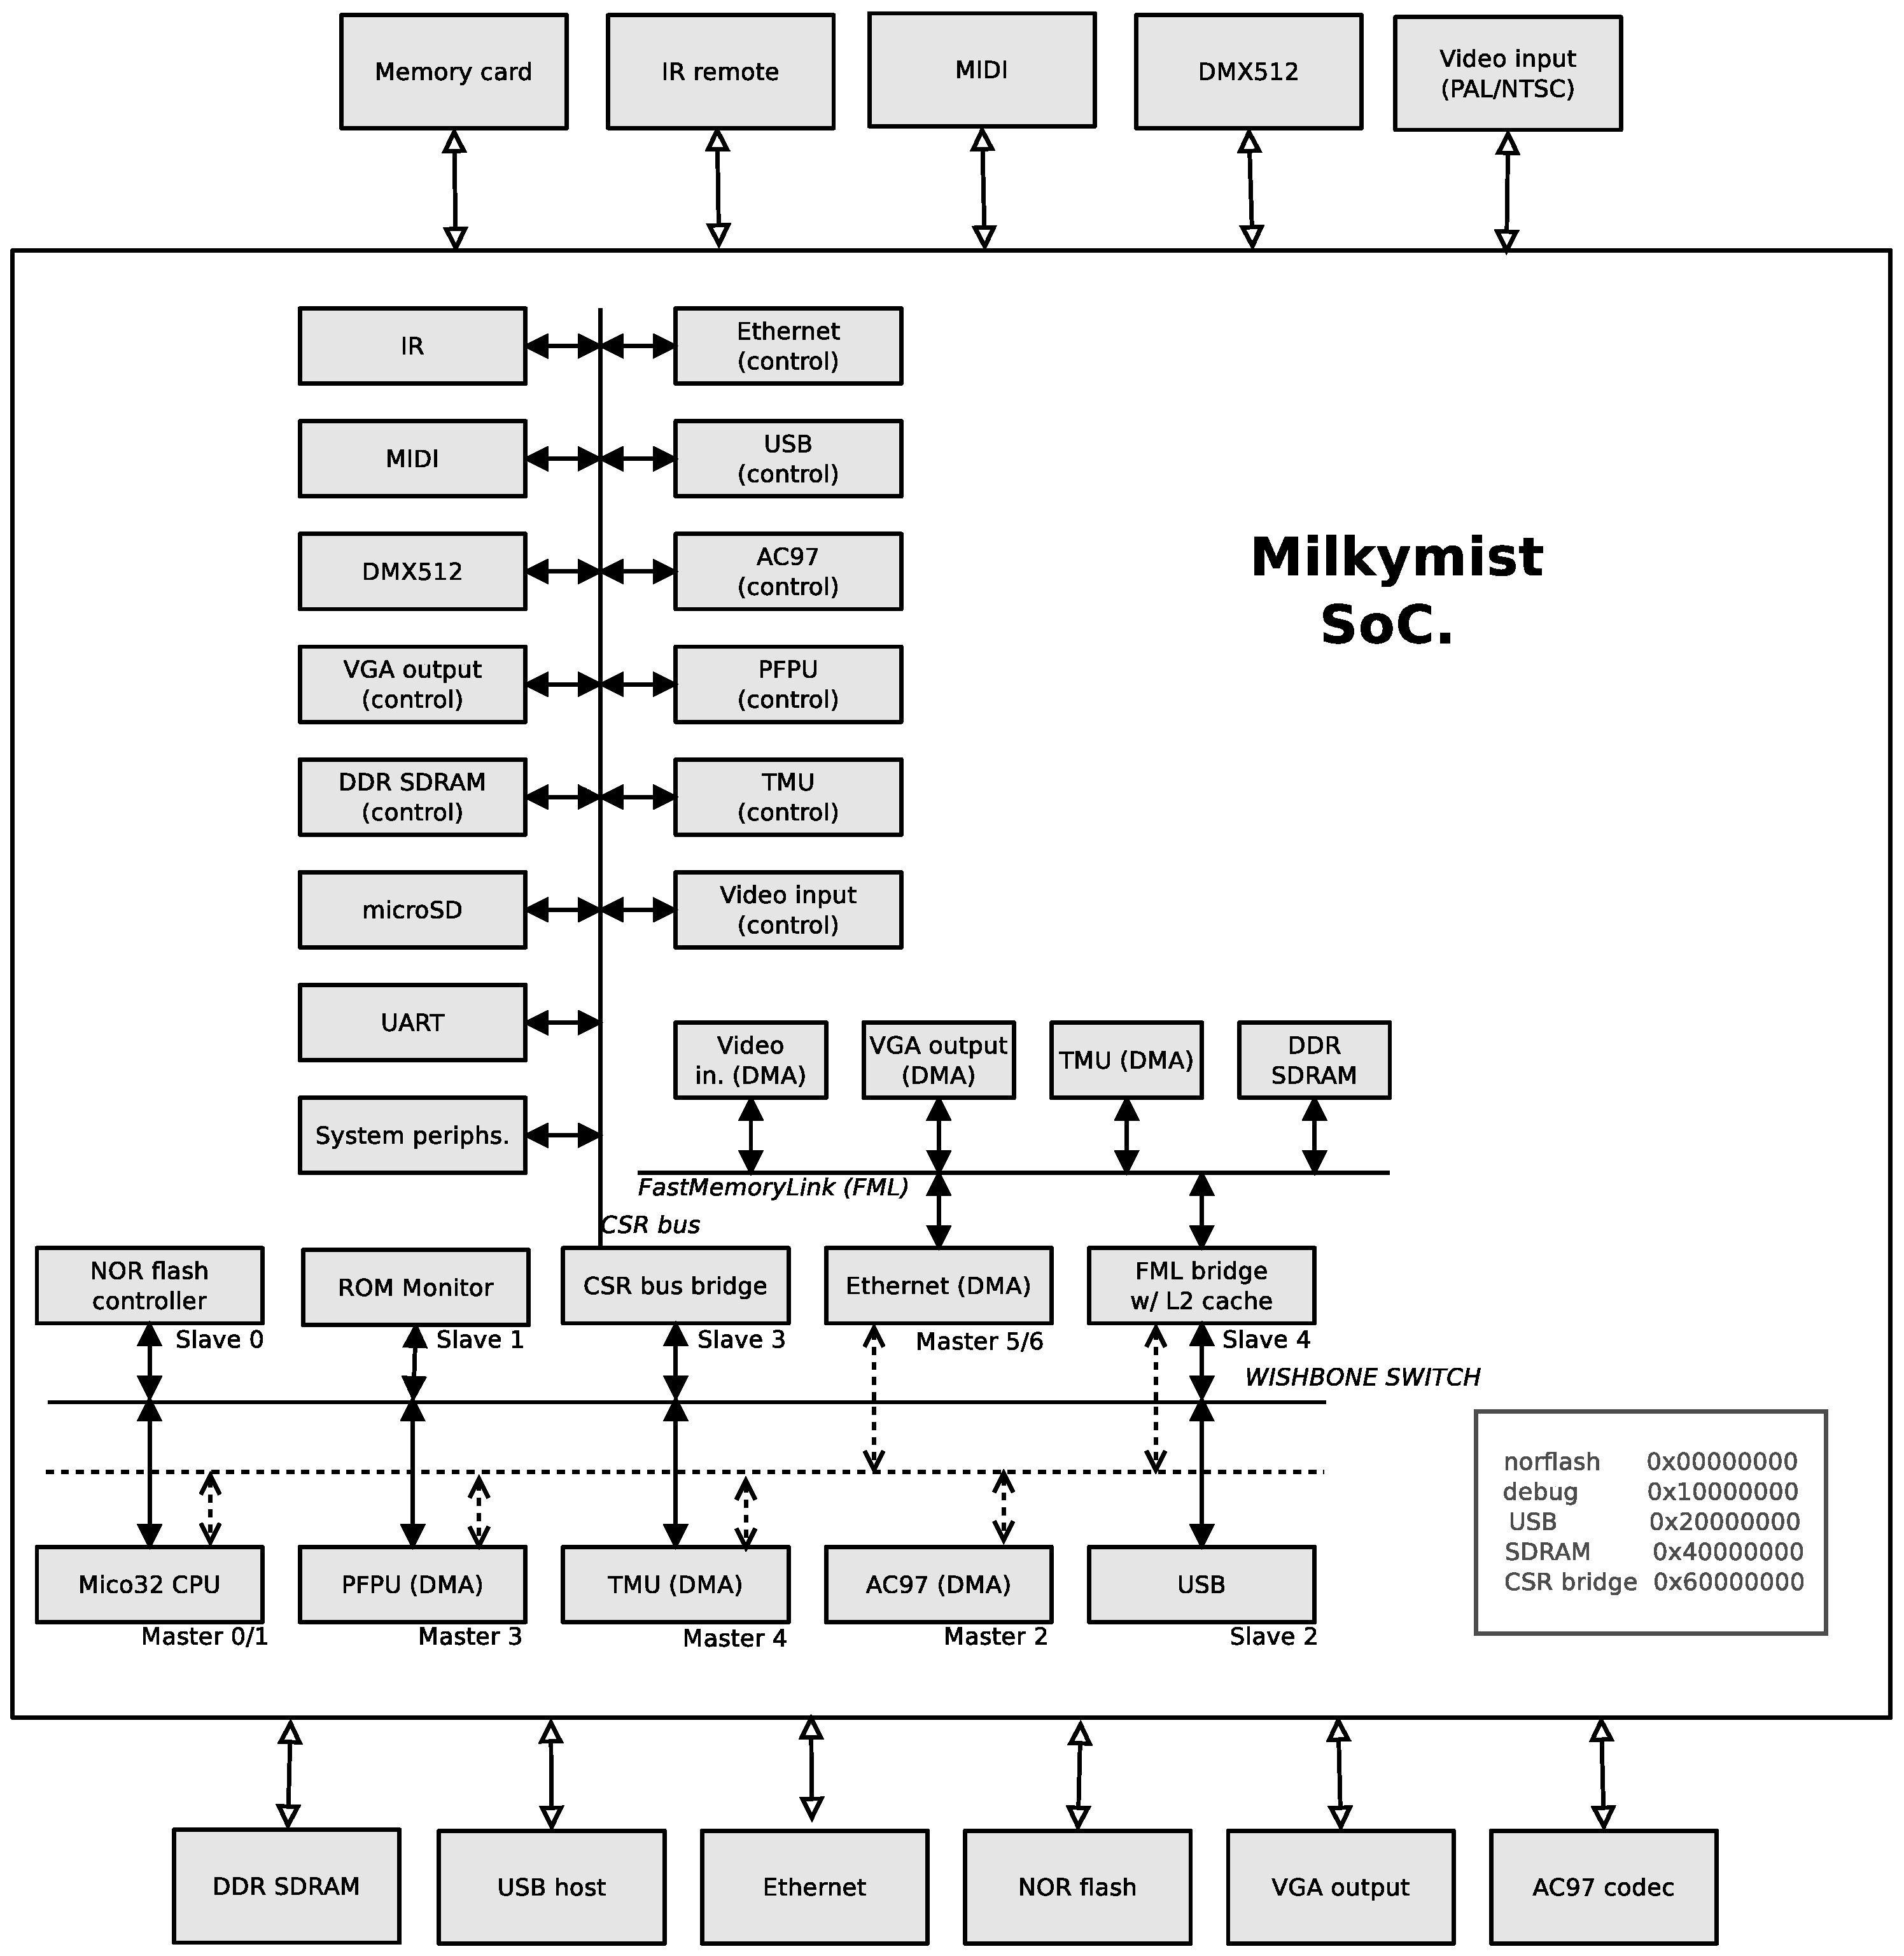
\includegraphics[height=130mm]{soc_architecture.eps}
\caption{SoC block diagram}
\end{figure}

\subsection{Softcore CPU}
The system is equipped with a small general-purpose CPU that drives the hardware acceleration units and performs software-friendly tasks such as GUI and filesystem handling.

Mico32 from Lattice Semiconductor has been chosen for this purpose. It can run a special MMU-less version of Linux, and the Milkymist BIOS supports direct loading and booting of Linux kernels.

\subsection{System memory}
\subsubsection{NOR flash}
The Milkymist BIOS is stored in an external NOR flash chip. The NOR flash controller in Milkymist has been designed to prioritize hardware simplicity over performance and functionality. It only supports reading from the flash; storing the boot image must be done using another tool.

\subsubsection{On-chip SRAM}
The SoC is equipped with a 4KB on-chip RAM, which is mainly used for the initial execution environment, before SDRAM is initialized and functional.

The choice has been made to include this on-chip RAM so that advanced debug programs that do not rely on SDRAM can easily be developed and run. Those programs are very useful for debugging the SDRAM, which is often prone to problems.

\subsubsection{SDRAM}
For large volatile data storage, Milkymist is designed to use affordable and industry-standard DDR SDRAM chips. A custom memory controller (HPDMC) has been designed as part of the project, as all other free cores were either non-functional or slow.

The memory controller implements the proprietary high-performance FML bus to deliver low-latency and high-bandwidth memory access while using few FPGA resources. FML has been designed as part of the Milkymist project.

\subsection{UART}
A simple UART is included, intended to implement a debug console. The UART parameters are fixed: 115200 bps, 8 bits per character, no parity, 1 stop bit.

\subsection{System controller}
The design uses a ``system controller'' core which includes the interrupt controller, GPIO, two timers, and a 32-bit identification number for the board.

See the ``GPIO maps'' and ``IRQ maps'' sections for GPIO and IRQ assignments.

\subsection{Memory card}
On the ML401, the CF card is accessed through the Xilinx SystemACE chip. The registers of this chip are mapped in the softcore CPU address space using the WISHBONE bus.

\subsection{VGA controller}
Milkymist uses a VGA signal generator which reads from a RGB565 framebuffer, and implements an FML master to fetch data from the memory. The VGA generator is controlled using a CSR interface.

\subsection{Audio}
Milkymist can record and play audio through an AC'97 codec. The core that drives the codec is controlled via a CSR interface and supports DMA reads and writes of the PCM data over Wishbone.

\subsection{Programmable Floating Point Unit (PFPU)}
The PFPU is a simple and high-speed floating point microprocessor, designed to do the bulk vertex data generation for each frame in little time.

It has a WISHBONE master for writing the output buffer, and a CSR interface for control.

\subsection{Texture Mapping Unit (TMU)}
The engine performs texture mapping on a triangle strip. It is a central component of MilkDrop acceleration.

It has two FML master interfaces for fetching pixel data, a WISHBONE master to fetch the vertex data, and a CSR slave for control.

\section{GPIO map}

\subsubsection{Inputs}

\begin{tabularx}{\textwidth}{|l|l|X|}
\hline
\bf{PIO bit} & \bf{Direction} & \bf{Description} \\
\hline
0 & Input & Pushbutton North \\
\hline
1 & Input & Pushbutton West \\
\hline
2 & Input & Pushbutton South \\
\hline
3 & Input & Pushbutton East \\
\hline
4 & Input & Pushbutton Center \\
\hline
5 & Input & DIP switch 1 \\
\hline
6 & Input & DIP switch 2 \\
\hline
7 & Input & DIP switch 3 \\
\hline
8 & Input & DIP switch 4 \\
\hline
9 & Input & DIP switch 5 \\
\hline
10 & Input & DIP switch 6 \\
\hline
11 & Input & DIP switch 7 \\
\hline
12 & Input & DIP switch 8 \\
\hline
\end{tabularx}

\subsubsection{Outputs}

\begin{tabularx}{\textwidth}{|l|l|X|}
\hline
\bf{PIO bit} & \bf{Direction} & \bf{Description} \\
\hline
0 & Output & LED 2 (NB. LED 0 and LED 1 respectively monitor UART transmission and reception) \\
\hline
1 & Output & LED 3 \\
\hline
2 & Output & LED North \\
\hline
3 & Output & LED West \\
\hline
4 & Output & LED South \\
\hline
5 & Output & LED East \\
\hline
6 & Output & LED Center \\
\hline
7 & Output & HD44780-compatible LCD -- E pin \\
\hline
8 & Output & HD44780-compatible LCD -- RS pin \\
\hline
9 & Output & HD44780-compatible LCD -- RW pin \\
\hline
10 & Output & HD44780-compatible LCD -- D4 pin \\
\hline
11 & Output & HD44780-compatible LCD -- D5 pin \\
\hline
12 & Output & HD44780-compatible LCD -- D6 pin \\
\hline
13 & Output & HD44780-compatible LCD -- D7 pin \\
\hline
\end{tabularx}

\section{Address map}

\begin{tabularx}{\textwidth}{|l|l|X|}
\hline
\bf{Base address} & \bf{Cacheable} & \bf{Peripheral} \\
\hline
0x00000000 & Yes & Boot ROM (NOR Flash) \\
\hline
0x20000000 & Yes & On-chip SRAM \\
\hline
0x40000000 & Yes & \textit{FastMemoryLink bridge} \\
\hline
\hspace{5mm} 0x40000000 & Yes & \hspace{5mm} DDR SDRAM data \\
\hline
\hspace{5mm} 0x44000000 & Yes (write-through) & \hspace{5mm} L2 cache line flush \\
\hline
0x80000000 & No & \textit{CSR bridge} \\
\hline
\hspace{5mm} 0x80000000 & No & \hspace{5mm} UART \\
\hline
\hspace{5mm} 0x80001000 & No & \hspace{5mm} System controller \\
\hline
\hspace{5mm} 0x80002000 & No & \hspace{5mm} DDR SDRAM control \\
\hline
\hspace{5mm} 0x80003000 & No & \hspace{5mm} VGA \\
\hline
\hspace{5mm} 0x80004000 & No & \hspace{5mm} AC'97 \\
\hline
\hspace{5mm} 0x80005000 & No & \hspace{5mm} PFPU \\
\hline
\hspace{5mm} 0x80006000 & No & \hspace{5mm} TMU \\
\hline
\hspace{5mm} 0x80007000 & No & \hspace{5mm} PS2 \\
\hline
0xa0000000 & No & SystemACE \\
\hline
\end{tabularx}

\section{IRQ map}
\begin{tabularx}{\textwidth}{|l|X|}
\hline
\bf{IRQ} & \bf{Peripheral} \\
\hline
0 & GPIO \\
\hline
1 & Timer 0 \\
\hline
2 & Timer 1 \\
\hline
3 & UART (RX)\\
\hline
4 & UART (TX)\\
\hline
5 & AC'97 (codec configuration registers, request sent)\\
\hline
6 & AC'97 (codec configuration registers, reply received)\\
\hline
7 & AC'97 (DMA read)\\
\hline
8 & AC'97 (DMA write)\\
\hline
9 & Programmable Floating Point Unit\\
\hline
10 & Texture Mapping Unit\\
\hline
11 & PS2 Interface\\
\hline
\end{tabularx}

\section{BIOS and boot process}
Using an ``execute-in-place'' schema, the system boots from the NOR flash, mapped at address 0x00000000 (the reset vector for the softcore CPU). It contains a BIOS which is in charge of booting the board as well as providing debugging features.

The Milkymist BIOS is based on FreeMAC (\url{http://lekernel.net/prism54/freemac.html}), originally written for running on the ARM embedded processors of Prism54 Wi-Fi cards. It has undergone major modifications since then.

The BIOS loads firmware from an external source (CF card or UART). The BIOS supports direct booting of Linux kernels. If no suitable boot medium is found, it starts a debug shell on the UART, which allows to do basic system operations such as writing to registers. The \verb!help! command lists the commands available with the BIOS release you are currently using.

All transmissions over the UART are made at 115200 bps or 230400 bps, with 8 bits per character, without parity, and with 1 stop bit. The second DIP switch on the board enables the 230400 bps rate when it is set, which is convenient when transferring large firmware images such as Linux kernels.

\subsection{Starting Linux}
The BIOS can directly start versions of Linux specifically made for running on Milkymist boards. Such modified Linux kernels are distributed separately.

\begin{itemize}
\item \textbf{The Linux kernel itself} is always loaded at the beginning of the SDRAM (0x40000000) and executed from there.
\item \textbf{Kernel command line parameters} are written to SDRAM and their address is set in CPU register \verb!r1! before the kernel is started.
\item \textbf{Initial ramdisk (initrd)} is optionally loaded into SDRAM and its start and end addresses are set in CPU registers \verb!r2! and \verb!r3!, respectively.
\end{itemize}

\subsection{Boot from the UART}
The first boot medium tried by the BIOS is the UART, using a special protocol. This enables firmware replacement during development by just connecting the serial cable and not switching a memory card between a computer and the device.

The device initiates an UART boot session by sending the ASCII string \verb!sL5DdSMmkekro! followed by a carriage return. This string is completely random, but has been encoded in ASCII so it does not garble the output of terminals which are not aware of the boot protocol.

Upon reception of this magic string, the UART boot program running on the host computer acknowledges it by returning the ASCII string \verb!z6IHG7cYDID6o! followed by a carriage return. This puts the device in firmware reception mode, and further commands are sent in binary using the protocol described below.

The host sends command to the device, which acknowledges them or reports errors by sending one ASCII character after each command. Those characters and their meanings are listed in the table below:\\

\begin{tabular}{|l|l|}
\hline
\verb!K! & Command successful \\
\hline
\verb!C! & CRC error, retry the command \\
\hline
\verb!U! & Unknown command ID \\
\hline
\verb!E! & Generic error \\
\hline
\end{tabular}\\

The host must wait for a reply from the device before sending the next command. However, it can retry the command after a timeout.

All the commands sent by the host are frames using this common format:\\

\begin{tabular}{|l|l|l|l|}
\hline
\textbf{Length} & \textbf{CRC16} & \textbf{Command ID} & \textbf{Payload} \\
\hline
1 byte & 2 bytes & 1 byte & 0-255 bytes \\
\hline
\end{tabular}\\

(As in the whole document, all multi-byte numbers are big-endian unless otherwise specified)

The length field is the length of the payload. The CRC16 is computed on the command ID followed by the payload.

The following commands are implemented:\\

\begin{tabularx}{\textwidth}{|l|X|}
\hline
\textbf{Command ID} & \textbf{Description} \\
\hline
0x00 & Abort session. No payload. The BIOS continues to the next boot medium. \\
\hline
0x01 & Load to memory. The payload is a 32-bit start address followed by the data. \\
\hline
0x02 & Jump. The payload is the 32-bit jump address. \\
\hline
\multicolumn{2}{|c|}{\textbf{Linux-specific commands}} \\
\hline
0x03 & Set Linux kernel command line parameters address. The payload is the 32-bit address. This address is written to the CPU register r1 before the kernel is started (using a jump command). \\
\hline
0x04 & Set Linux kernel initrd start address. The payload is the 32-bit address. This address is written to the CPU register r2. \\
\hline
0x05 & Set Linux kernel initrd end address. The payload is the 32-bit address. This address is written to the CPU register r3. \\
\hline
\end{tabularx}

\subsection{Boot from the CF card}
If the device has not received an acknowledgement for UART boot after a certain period of time, it then attempts to boot from the CF card.

For this purpose, it searches for a file named \verb!BOOT.BIN! on the first FAT partition. It then loads it into the beginning of the SDRAM, and, if this was successful, transfers execution to the SDRAM.

If the first DIP switch on the board is set, the BIOS uses the \verb!ALTBOOT.BIN! file instead.

\paragraph{Linux support.} If the CF card also contains files named \verb!CMDLINE.TXT! and \verb!INITRD.BIN!, they are loaded into SDRAM at offsets \verb!0x1000000! (16MB) and \verb!0x1002000! (16MB + 8KB) respectively. The addresses are then passed to the kernel (loaded from \verb!BOOT.BIN! or \verb!ALTBOOT.BIN!) using CPU registers \verb!r1!, \verb!r2! and \verb!r3! (see above). The files must be small enough so that they do not overlap in memory.

\end{document}
